%-------------------------------------------------------------------------------
%	CAPITOLO 41
%-------------------------------------------------------------------------------

\chapter{I due Capelli - Gioti}
\index[Personaggi]{Capelli (avvocato)}Uno affogato nel vino. Parliamo di quello. Era un valore come legale, conscio del suo valore ne era altero e soffriva mal volentieri di fare il suo tirocinio alle dipendenze di un celebre avvocato di \index[Luoghi]{Bologna}Bologna il quale trionfava nei Tribunali con le difese del nostro uomo.\\
L'applicazione allo studio, il mal trattamento od altro rovinarono la salute del nostro emerito avvocato... ed i genitori lo vollero a casa per guadagnare la salute.\\
Qui era medico primario il povero dott \index[Personaggi]{Gamberini Dr. Giulio}Gamberini, che aveva una grande fiducia nei buoni effetti rigenerativi del vino e cognac.\\
Avendo sotto la sua casa il nostro avvocato, esile, allampanato... senza appetito ed astemio, cominciò a farlo trincare per rinvigorirlo. Fu una sbornia attaccata all'altra e lo rovinò.\\
Solitamente la sbornia di carnevale cominciava in lui a Natale e finiva a Pasqua. Fiutava tabacco e chi lo avesse spolverato ne poteva ammassare qualche ettogrammo\footnote{Il protagonista era talmente impolverato che, scrollandolo, si poteva recuperare qualche ettogrammo di tabacco}.\\
Il povero avvocato era ridotto ad uno stato miserevole dagli aiuti dell'alcool... in mezzo ad una festa da ballo, nella piazza affollata orinava in faccia al pubblico...\\
Se la prendeva coi pretori perché non gli davano la vittoria nelle cause. I suoi ritornelli ed invettive ai principali pretori, chi non li ricorda?
\textcal{	
\begin{center}
\Huge
No, anavoi Capolozzo! Capolozzo!\\
No, anavoi Mambrucon\footnote{Mambrucone fu pretore ad Alfonsine. Citando Romano Pasi: "Questo pretore Scognamiglio, principe meridionale, soffriva molto il freddo alfonsinese, per cui ascoltava le parti in causa standosene al calduccio del letto, mentre al cancelliere faceva mettere tutto agli atti. Quando la corte si ritirava per deliberare, si tirava la coperta sul capo, e dopo un po', scoprendo il volto, emetteva la sentenza."}!\:\:\footnote{"No, non voglio Capolozzo! Capolozzo; No, non voglio Mambrucone!"}
\end{center}}
\index[Personaggi]{Capolozzo}\index[Personaggi]{Mambrucone (pretore)}
\normalfont \normalsize
\noindent Di lui era caratteristica la macchietta.\\
Ecco l'uomo colto... ridotto incolto... dall'alcool.
 \begin{figure}[htb]
    \centering
    %\vspace{-0.7cm}
    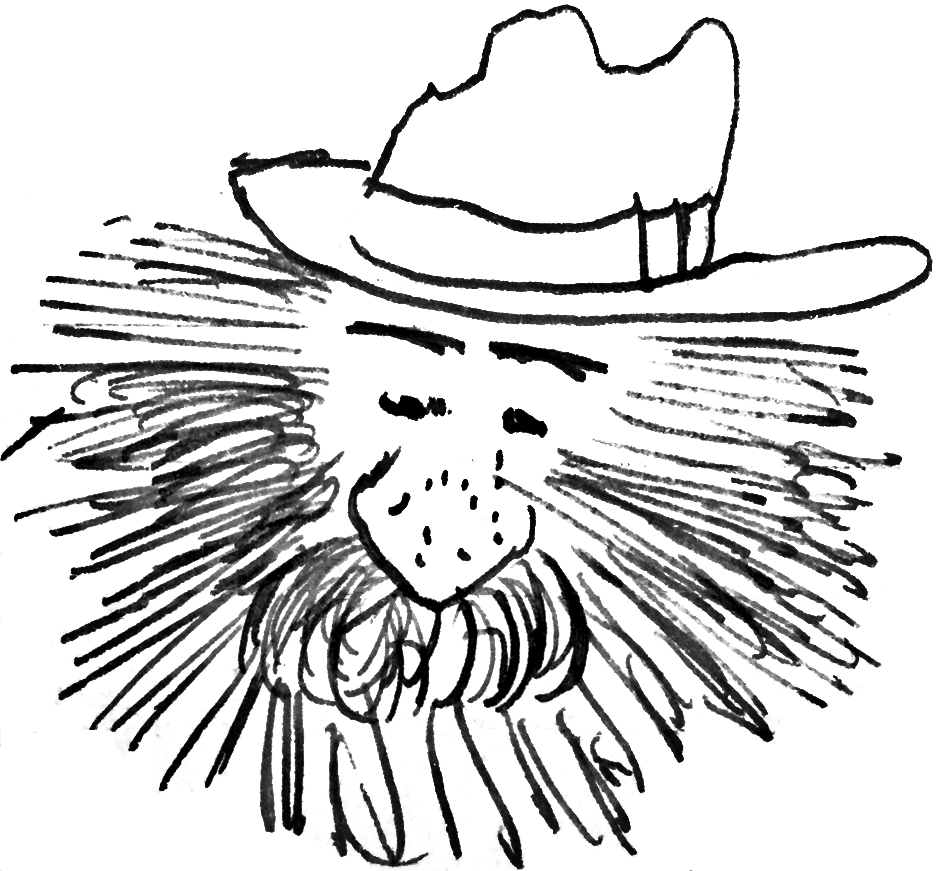
\includegraphics[height=6cm]{Capelli_Avvocato}
    %\vspace{-0.3cm}
\end{figure}\newpage
\index[Personaggi]{Capelli (protocollista)}
\noindent Sotto l'altro\footnote{E ora parliamo dell'altro}. \\Per questo la gola fu fatale. I tortelli hanno ucciso Capelli, questa orrenda notizia vi dò!\\
Tipo curioso, si credeva bello irresistibili alle donne. Permaloso, un pò tardo di comprendonio sotto lo sforzo della digestione.\\
Offriva a tutte le belle ragazze 100 scudi per una gita... con lui a \index[Luoghi]{Ravenna}Ravenna. Distribuiva a 60 anni, alle sue dame il suo ritratto all'età di 20 anni, vestito da sottotenente, nella sua caratteristica figura. La faccia sembrava una gran luna con sopra un guscio d'ovo, che era il berretto, due baffetti spioventi alla cinese, occhini coperti da grosse palpebre, sembrava un maiale della grassa. \\
Si riteneva molto eloquente, faceva il causidico\footnote{Avvocato da poco} in pretura ed una volta presentò una comparsa con citazioni latine... che non conosceva. Il Pretore \index[Personaggi]{De Simone (pretore)}De Simone, ebbe a dirgli: "Ecco spieghi questa..."\\
Al nostro causidico cadde il mondo addosso e credè rispondere: "Ecco... si... già... s'intende..." e fu una risata generale.\\
Aveva lo stipendio da protocollista in comune, ma il suo tempo era diviso per le seguenti funzioni:\\
\begin{itemize}
\item[9.00]purga con acqua - Janos\footnote{Acqua medicinale Hunyadi János, conosciuta e consumata dal 1863, costituita da sale di Glauber e sale inglese.}
\item[10.00]leggere sotto lo scaffale della scrivania il giornale, e brontolare a chi osava varcare la porta del suo ufficio: "Ho da fare lasciatemi in pace..."
\item[11.00]entrata nella vecchia latrina del palazzo comunale, dove c'era una gran pietra per posare i piedi, dietro una buca di m. 1,50 per 0,80 e dopo il muro.\\
Giù le brache... chino il corpo in orizzontale, non arrivava ad accovacciarsi sui polpacci... che la scarica avveniva nel muro di contro con una rosa di almeno 60 centimetri. \\
Chi andava dopo di lui vedeva i segni di \index[Personaggi]{Capelli (protocollista)}Capelli
\item[11.30]Andava alla firma, riceveva 4,5 lettere da protocollare.
\item[12.00] a mangiare.
\item[13.00] a fare il chilo sul sofà e respirare a due riprese, perché troppo pieno.
\item[13.30] per la strada presso le fruttivendole a mangiare arance, mele, mandarini, zucca cotta ecc.
\item[14.00] all'ufficio a cominciare missive d'affari sui grandi fogli da protocollo, poi accartocciava tutto... perché sbagliava perché era troppo pieno... e non concepiva il pensiero.
\item[17.00] (d'inverno) uscito dall'ufficio, passava a rifornirsi di cioccolatini e poi da qualche bella a farseli mangiare.
\item[18.00](se d'estate) all'osteria a ordinare un etto di mortadella, o salame, mezzo litro, e due soldi di pane, con molti bis.
\item[19 - 20] a cena a divorar tutto.
\item[20.30] al caffè cominciava a bere latte mangiar paste, biscotti, pan di Spagna ecc. per qualche mezzo chilo.
\item[21.30] a morosa fino alle 22
\item[22.00] entrato nell'osteria annusava come un cane da trifola , poi chiedeva : "Che cosa hai rimasto?"\\
Oste: "Cappelletti, umido, arrosto, lesso."\\
\index[Personaggi]{Capelli (protocollista)}Capelli: "Fammi vedere" poi "Quanto vuoi per tutto?"	\\ Il contratto era fatto e tutto divorato.
\item[23.00] Chiudevano l'osteria ed il nostro uomo prendeva la via dell'amata... fino alle una,,, a fare il chilo e farsi far vento alla pancia perché gli tirava per avere troppo mangiato...
\item[1.00] tornava a casa e dava aria ai polmoni... ed alla strada... per sgonfiare la pancia. Poi a letto fino alle 8.
\end{itemize}
Era assiduo di tutti gli spettacoli ai quali assisteva divorandosi brustole\footnote{Semi di zucca}, caramelle, cioccolatini ecc.\\
Credeva di conquistare le commedianti o cantanti, ronzando sempre loro intorno come un molesto bagarone\footnote{Calabrone}... Una sera il pover'uomo era a godersi uno spettacolo, seduto su una delle prime fila di sinistra del \index[Luoghi]{Baraccone (teatro)}Baraccone. Aveva mangiato più del solito, la sua testa era in confusione credendosi ammirato... (e per questo era abile perché aveva una gran cura di mostrare alle artiste il portafoglio e di promettere molto...) ma la digestione lo disturbava molto e lo assopiva. Però non poteva né assopirsi né sedersi comodamente... era come sugli spini per la gonfiezza. Sulla fine di un atto uscì, si appressò alla siepe del \index[Luoghi]{Carraretto Venturi}Carraretto\footnote{Carraretto Venturi, il teatro fu spostato nel Carraretto Venturi (e lazarètt) già dal 1894}, ad orinare quando credé di fare uno sforzo per vuotare l'aria... ma il colpo fu tale e forte... da prendere una lombaggine\footnote{Dolore in sede lombare che si acutizza nei movimenti di flessione ed estensione del tronco} ("snestar"\footnote{Espressione dialettale per `colpo della strega'}) e dovettero portarlo a casa, e chiamato il povero \index[Personaggi]{Novi (dottore)}Dr. Novi e l'infermiere \index[Personaggi]{Domenico Soatti, Mingò d'Galèna (infermiere)}Mingone di Gallina, che lo sottoposero ad una iniezione calmante. \\
Era sempre tutto gentile... per non far torto al suo budello\footnote{SISTEMARE} idem che tanto lo aiutava. Era geloso di tutti e di tutte.\\
Il povero \index[Personaggi]{Isani Nando (farmacista)}Nando Isani, aiuto farmacista da \index[Personaggi]{Boari Attilio (farmacista)}Boari, quando lo vedeva venire serrava la bussola\footnote{Portantina} della farmacia e si nascondeva nel laboratorio.\\
Cominciava allora la scena da ridere. \index[Personaggi]{Capelli (protocollista)}Capelli, spingeva la bussola, chiamava... strimpellava, perché si metteva in sospetto che nel retro farmacia Nando \index[Personaggi]{Isani Nando (farmacista)} avesse qualche avventura galante... e lui voleva sorprenderlo... per intimare alla femmina... amore anche per lui... \\
La porta rimaneva chiusa e \index[Personaggi]{Capelli (protocollista)}Capelli guardia portone, finché dopo un gran pezzo appariva il povero Nando \index[Personaggi]{Isani Nando (farmacista)} facendo l'imbronciato, e cominciava il dialogo.\\
Capelli: "Chi avevi..."\\
Nando: "Nessuno, che cosa vuol sapere!"\\
Capelli: "Va là dimmelo, ti vuoi godere solo tu... ed insisteva per delle ore..."\\
Capelli a qualche altro: "Mo chi era la donna, dove è?"\\
Interrogato: "Stia zitto è scappata dalla porta di dietro!"\\
Capelli: "Porca, non sono capace di trovarla!"\\
E la commedia si ripeteva spesso... tra le risate.\\
Una delle sue amate stava in \index[Luoghi]{Vincenzo Monti (piazza)}Piazza\footnote{Piazza Monti} di fronte al \index[Luoghi]{Palazzo Comunale}Palazzo Comunale ed aveva le finestre al 2° piano.\\
\index[Personaggi]{Capelli (protocollista)}Capelli si metteva alla finestra del \index[Luoghi]{Palazzo Comunale}Palazzo Comunale, la sua amata... alla sua, distante 150 metri e pretendeva di essere ammirato. Una volta poi avvenne che i saltimbanchi eressero in \index[Luoghi]{Vincenzo Monti (piazza)}Piazza grandi tende ed impedirono l'idillio di ammirazione. Il nostro \index[Personaggi]{Capelli (protocollista)}Capelli se la prese con l'amata... e la piantò per qualche tempo.\\
L'amata però mal soffriva un tale ingiusto trattamento e decise di fermare l'amato bene un sera quando andava a casa. Il colloquio si svolse così:\\
Amata: "Perché non vieni più?"\\
Capelli: "Perché non mi hai guardato dalla finestra..."\\
Amata: "Ma come devo fare, ci sono le baracche in mezzo e non si può vedere..."\\
Capelli: "A na voi savé me, va dsò da la Pia... (al 3° piano) me a voi t'am guerda"\footnote{"Non lo voglio sapere io, va di sopra dalla Pia, io voglio che tu mi guardi"}.\\
\newpage

\noindent Ammiriamo anche noi questo pachiderma.
 \begin{figure}[htb]
    \centering
    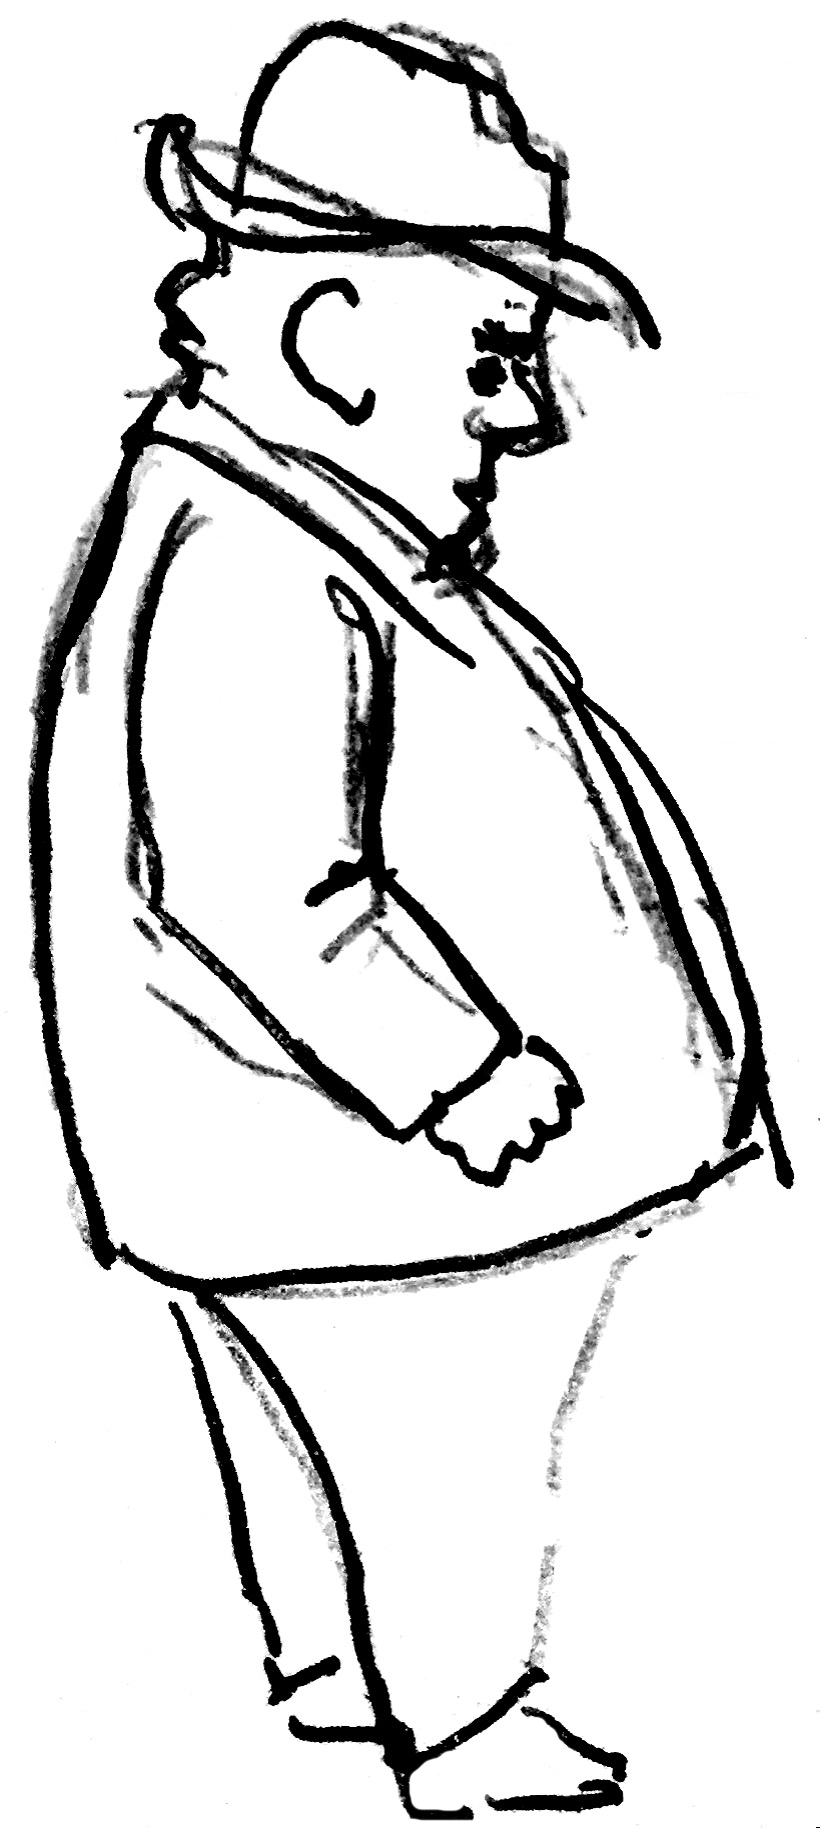
\includegraphics[height=12cm]{Capelli_mangione}
    %\vspace{-0.3cm}
\end{figure}

\newpage
Teneva regalare copia e minute\footnote{Le prime stesure provvisorie delle lettere} delle lettere amorose che riceveva, la collezione dei ricciolini... e di altri peli ancor più fini...\\
Dopo morto si trovò tutto questo materiale documentario della sua attività conquistatrice ed una cambiale, con la firma del povero \index[Personaggi]{Capelli (protocollista)}Capelli ed altra persona con accompagnato un biglietto così concepito:
\begin{center}
	\emph{Caro Capelli, vi mando la cambiale che avete firmato per me, che ho pagato, e che ora ha solo un valore di riconoscenza. Vi prego di distruggerla, perché se la trovano i vostri eredi diranno che vi siete mangiati anche quelli...}
\end{center}
\:
\:
\subsection{Gioti}
Questo capitoletto è presente nell'indice, ma non fu mai scritto.\\
\begin{figure}[!htbp]
   \includegraphics[width=\textwidth]{"Gioti".jpg}
\end{figure}
\\Probabilmente Mingazzi voleva scrivevere qualche racconto su \index[Personaggi]{Marchiani Luigi `Gioti'}Marchiani Luigi (08/06/1872 - 29/04/1934). Alcuni vecchi del paese ancora lo ricordano, sempre a spasso con il suo asinello.

Riporto la prima pagina del racconto su Gioti della mia cara amica Hedda Forlivesi.\\

 \begin{figure}[htb]
    \centering
    %\vspace{-0.7cm}
    \includegraphics[width=\textwidth]{Gioti2}
    %\vspace{-0.3cm}
\end{figure}


